\documentclass[a4paper, UTF8]{ctexrep}
\usepackage{ctex}
\usepackage{amsmath}
\usepackage{multirow}
\usepackage{amssymb}
\usepackage{graphicx}
\usepackage{geometry}
\usepackage{bm}
\usepackage{subfigure}
\usepackage{float}

\renewcommand\thesection{\arabic{section}}

\begin{document}
	\begin{titlepage}
		\centering
		\vspace{6cm}
		\LARGE{图像处理中的数学方法第一次作业报告}\\
		\vspace{3cm}
		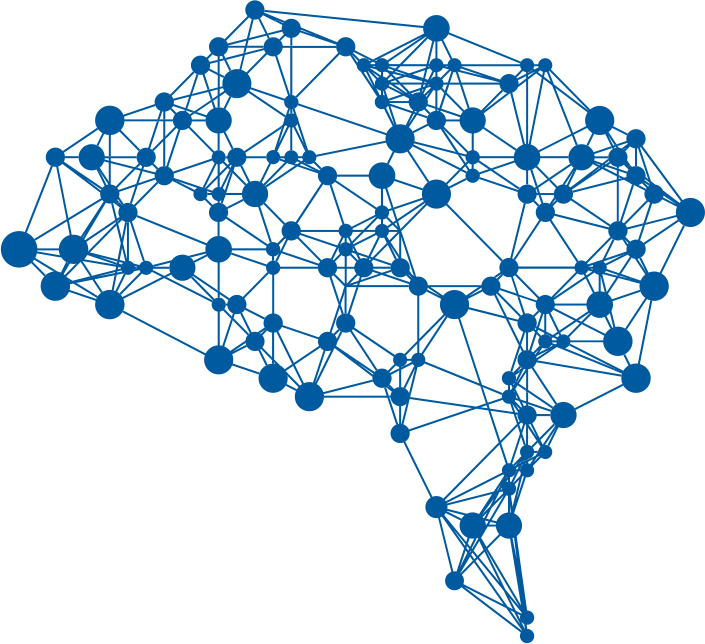
\includegraphics[width=0.8\textwidth]{deepLearning.png}\\
		\vspace{4cm}
		\normalsize{安捷 1601210097}\\
		\normalsize{\today}
	\end{titlepage}
	为了实现本次作业的需求,我基于MATLAB,实现了ADMM算法,利用迭代方法实现了去模糊+去噪的图像重建任务。下面从算法简述,参数设置,数值实验结果,结论四个方面总结本次作业。
	\section{算法简述}
		\begin{figure}
			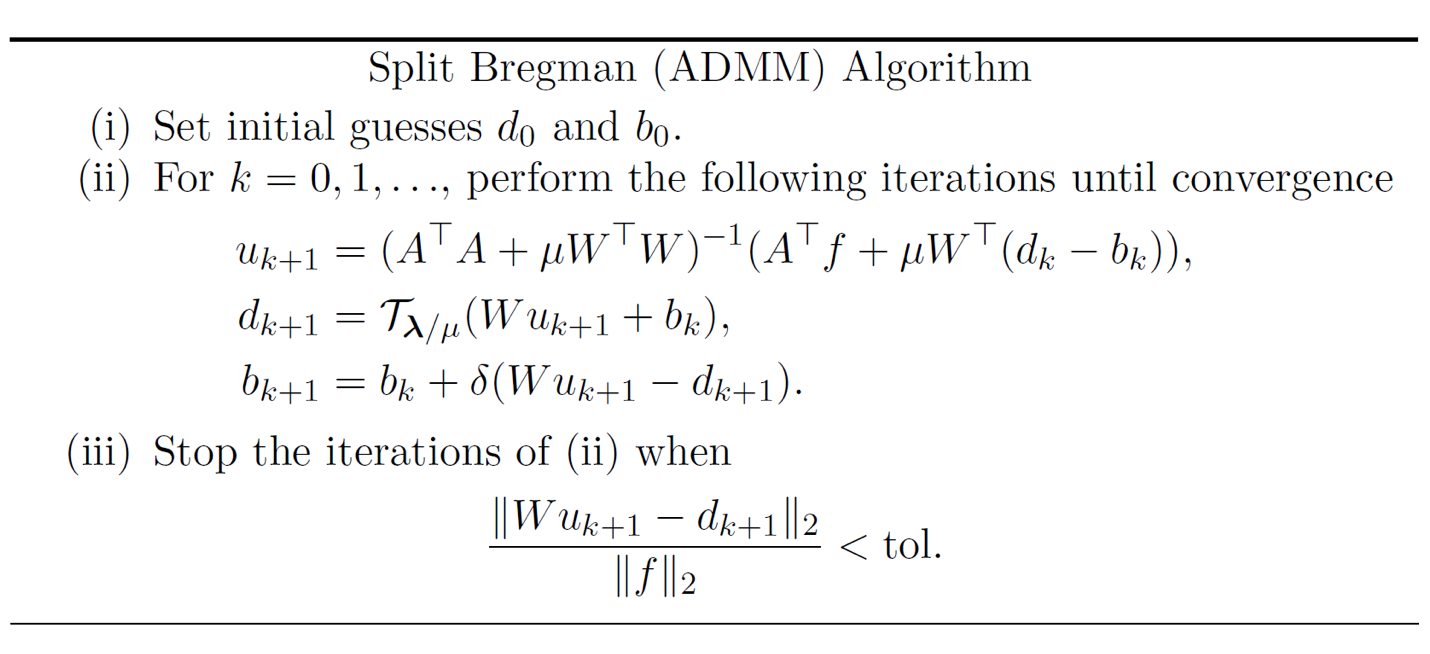
\includegraphics{fig1.png}
			\caption{算法流程}
			\label{}
		\end{figure}
		其中,主要问题在于第一步,在这次作业的开始,我尝试使用线性化的思路来实现本次作业,即,将 $A$算子与 $W$算子实现的操作转化为一个矩阵,经过线性化之后,上述流程中的操作全部转化为矩阵与向量的操作,这一操作可行,但是存在很严重的两个问题:
		\begin{enumerate}
			\item 存储困难,线性化的操作使得矩阵 $A$ 与$W$ 的维数是原图像的平方,即128*128的图像需要的双精度存储量为约1200MB,512*512的图像需要的双精度存储量为约80GB,如果不采取稀疏矩阵存储方式,几乎不可存储;
			\item 计算耗时长,在我使用的基于NVIDIA CUDA的GPU加速技术之后,依然速度很慢,主要原因在于矩阵求逆操作到目前为止没有效率很高的快速计算方法,即使采用GPU加速技术;
		\end{enumerate}
		基于以上两点原因,我放弃了这一方法,转为采用老师上课提到的利用Fourier Transform求解Possion方程的算法来求解ADMM算法的第一步。下面将算法简述如下:
		\begin{enumerate}
			\item 
		\end{enumerate}

\end{document}
